\begin{figure}[h]
    \centering
    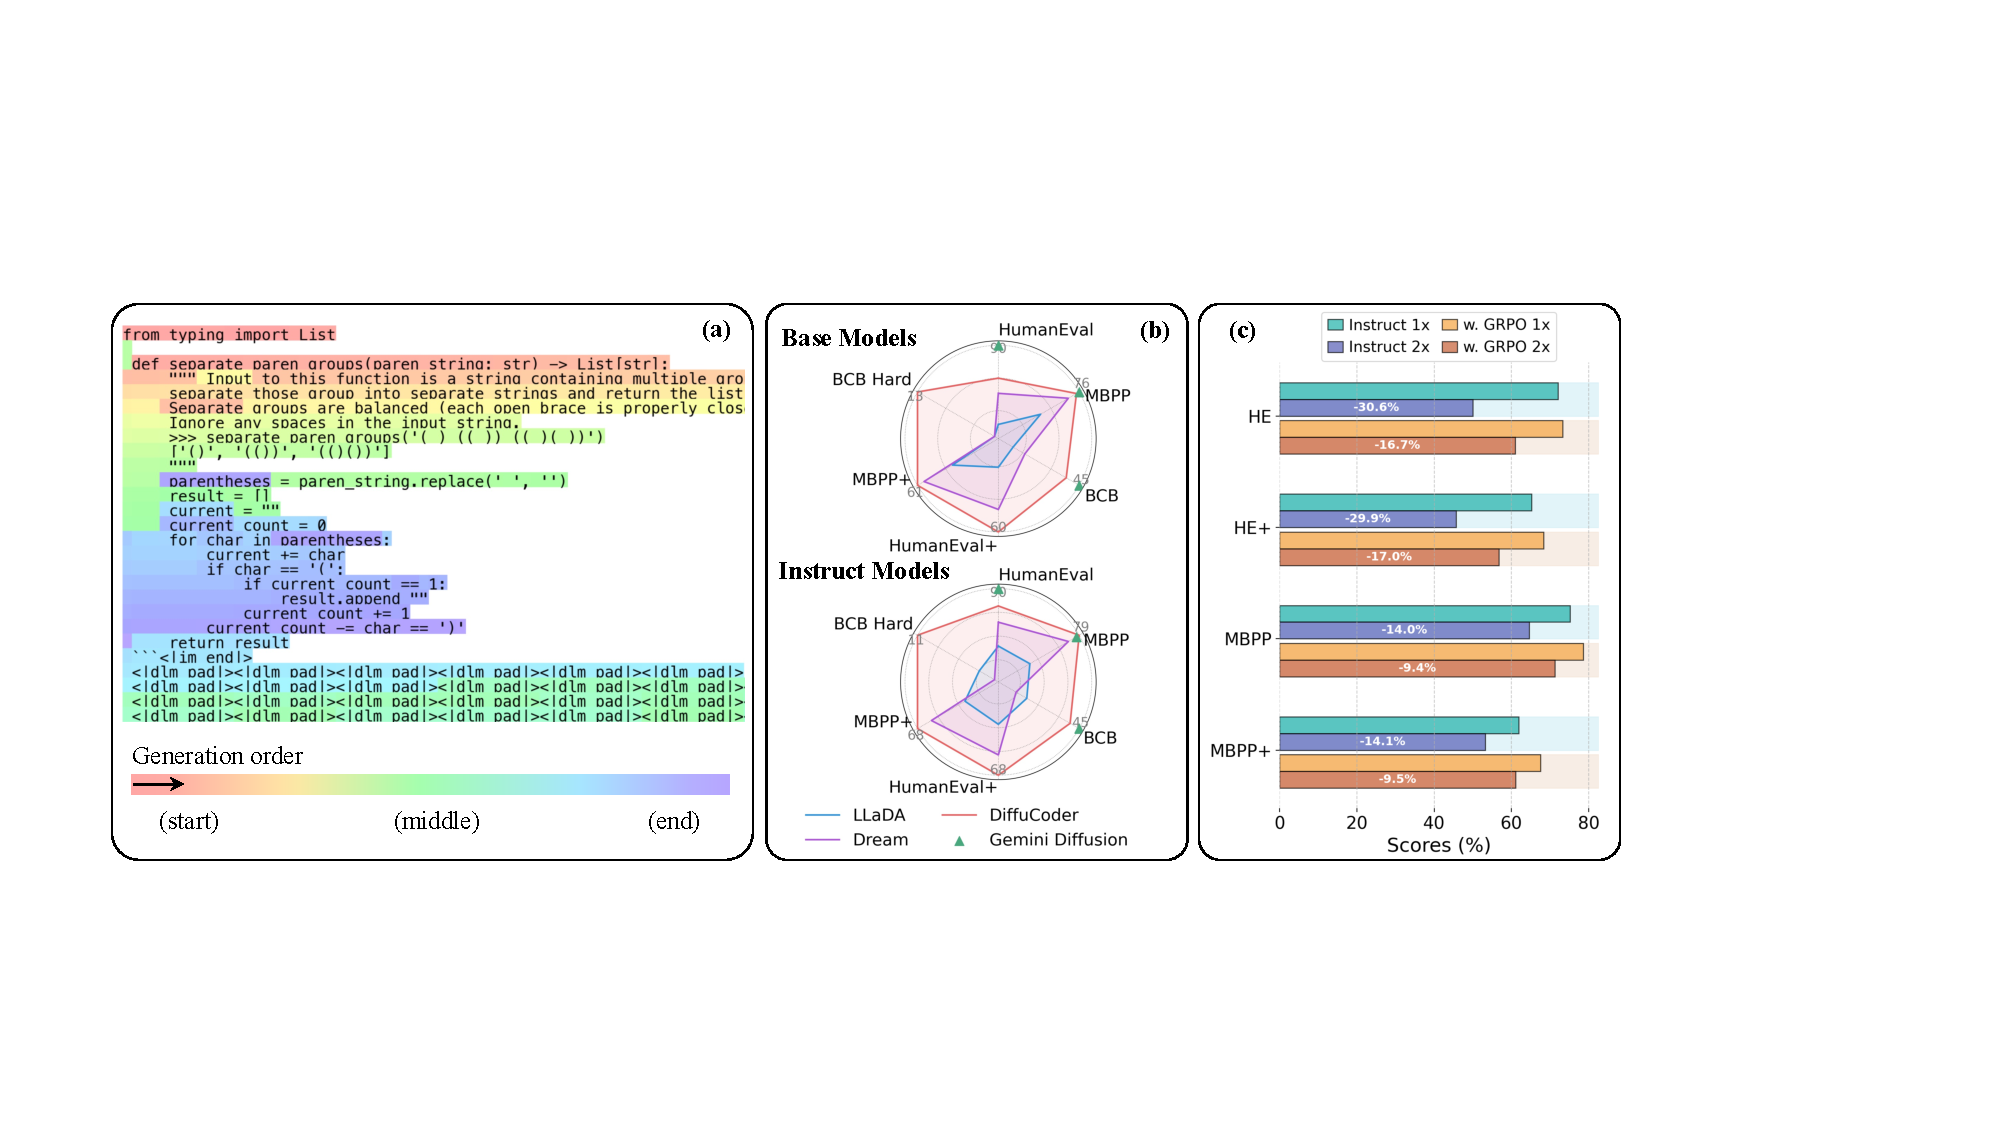
\includegraphics[width=1\linewidth]{fig/teaser2.pdf}
    \caption{(a) A real example of DiffuCoder-Instruct's decoding process with sampling temperature $1.2$. (b) Results on coding benchmarks. (c) When decoding steps are halved, DiffuCoder-Instruct trained with coupled-GRPO experiences a smaller performance drop, compared to Instruct itself.}
    \label{fig:teaser}
\end{figure}
\section{Introduction}

Large language models (LLMs) have revolutionized natural language processing, achieving remarkable results across tasks from dialogue to code generation~\citep{touvron2023llama,gpt4}.
While these successes are built predominantly on the autoregressive (AR) paradigm, masked diffusion models (MDMs) have recently emerged as a compelling alternative~\citep{Zheng2023ARD,shi2024simplified,sahoo2024simple}, and are further scaled to diffusion LLMs (dLLMs) like LLaDA~\citep{nie2024scaling} and Dream~\citep{dream2025}, which achieve performance on par with similarly sized AR LLMs.
Rather than generating left-to-right, MDMs iteratively refine the entire sequence in parallel, which allows for global planning of content~\citep{ye2024autoregressiondiscretediffusioncomplex,zhang2023planner}.

Intuitively, code generation aligns well with the dLLM paradigm, as writing code often involves non-sequential back and forth refinement~\citep{xie2025teaching}.
Recent commercial-scale dLLMs, Mercury~\citep{inception2025mercury} and Gemini~\citep{geminidiffusion}, show that a diffusion-based code generator can rival top AR code models. 
However, it remains unclear how open-source dLLMs perform on coding tasks, as their training and inference mechanisms are not yet fully interpreted.
Existing post-training efforts for dLLMs, such as LLaDA1.5~\citep{li2025llada} with DPO~\citep{rafailov2023direct} training, and d1~\citep{zhao2025d1}, MMaDA~\citep{yang2025mmada} with GRPO~\citep{shao2024deepseekmath} training, either show marginal gains or rely heavily on semi-AR decoding (\textit{i.e.}, block decoding with a relatively small block size; see~\citealp{arriola2025block}) which deviates from the global planning nature of diffusion. 
% Despite this intuition, the decoding behavior of dLLMs still lacks systematic investigation.
To address these limitations, we first gain insight into decoding behaviors of dLLMs and then establish a diffusion-native reinforcement learning (RL) methodology.

Our investigation is grounded in the analysis of \textbf{DiffuCoder}, a 7B-scale MDM specialized for code generation (\S\ref{sec:diffucoder}), trained on 130B effective tokens~\citep{huang2024opencoder}. The model's performance is competitive with that of AR coders, providing a strong testbed for understanding the behaviors of dLLMs and for developing diffusion-native post-training approaches.

To leverage the benefits of non-autoregressiveness in dLLMs, it is important to understand how non-autoregressive the behavior of current dLLMs actually is. To this end, we introduce local and global \emph{autoregressive-ness} (AR-ness) metrics (\S\ref{sec:metricdefine}) to measure how closely their generation follows a left-to-right pattern. 
Our analysis reveals that dLLMs exhibit an \emph{entropy sink} phenomenon (\S\ref{sec:analysis}), which causes a strong causal bias during conditional generation using low-confidence remasking decoding~\citep{maskgit}. We show that DiffuCoder can automatically decide how non-autoregressive it needs to be during decoding. When the sampling temperature is increased from the default $0.2$ to $1.2$, DiffuCoder becomes more flexible in its token generation order, freeing itself from strict left-to-right constraints, as Figure~\ref{fig:teaser}(a) shows. 
Unlike AR models, which primarily diversify token choices at higher temperatures, dLLMs additionally diversify the position of the generated token. 
With this increased diversity, DiffuCoder achieves higher pass@10 accuracy by changing the sampling temperature from $0.2$ to $1.2$ in our experiments (\S\ref{sec:gen-diver}). 
% This indicates that DiffuCoder has the potential for better performance and deserves\yz{I suggest changing "deserves" to "can benefit from"} effective RL exploration in the post-training stage.
The gain in pass@10 indicates the potential capacity of DiffuCoder, suggesting it can benefit from effective RL training to ``elicit out'' the most successful rollout samples.

Following this, we tailor GRPO~\citep{shao2024deepseekmath} for dLLMs. Our design focuses on reducing variance while maintaining efficiency in Monte Carlo estimations of token likelihoods. Specifically, we propose \textbf{coupled-GRPO}, which employs a novel coupled-sampling scheme. In detail, it adds paired complementary mask noise to the completion sequences generated by the model at a temperature of $1.2$. Unlike previous approaches~\citep{zhao2025d1}, our method does not rely on semi-AR decoding and it further improves the instruct-tuned model. After coupled-GRPO training, the model exhibits a stronger non-AR generation pattern, as inferred from Figure~\ref{fig:teaser}(c).

In summary, our contributions are as follows.
\begin{itemize}[leftmargin=13pt]
    \item We introduce a 7B dLLM for code generation, providing a foundation for developing diffusion-native training methods (\S\ref{sec:diffucoder}).
    \item We introduce local and global \emph{AR-ness} metrics to demystify the decoding patterns of dLLMs and track how AR-ness evolves across different training stages (\S\ref{sec:analysis}). Our analysis reveals that higher sampling temperatures encourage more parallel, non-AR generation (\S\ref{sec:gen-diver}).
    \item We design coupled-GRPO, an RL algorithm for dLLMs that avoids semi-AR decoding by using a novel coupled-sampling scheme for efficient and accurate policy gradient estimation (\S\ref{sec:grpo}). We theoretically prove the variance reduction of coupled-GRPO using antithetic variates.
    \item Experimentally, coupled-GRPO significantly improves DiffuCoder's performance, boosting its EvalPlus score by 4.4\% with training on only 21K samples and demonstrating the effectiveness of RL aligned with diffusion principles.
\end{itemize} 